\chapter{Raspberry Pi}

\section{¿Por qué Raspberry Pi?}

La utilización de una Raspberry Pi en este proyecto son claras y comentadas con anterioridad. 
Es un dispositivo de un tamaño muy reducido y portátil, que nos facilita mucho el poder llevarla a cualquier lugar sin dificultades y poder ofrecer un servicio en cualquier lugar.
Tiene unas prestaciones más que aceptables para un dispositivo de ese tamaño, conexiones inalámbricas como serian Wifi y Bluetooth integrados cosa impredecible para las comunicaciones con los sensores. Todo a un precio muy atractivo el cual permite su compra.  

Algunas de las especificaciones mas importantes de las Raspberry Pi 3 son las siguientes:
\begin{itemize}
\item 1.2GHz 64-bit quad-core ARMv8 CPU
\item 802.11n Wireless LAN
\item Bluetooth 4.1 y Bluetooth Low Energy (BLE)
\item 1GB RAM
\item Ethernet port
\item Micro SD card slot 
\end{itemize}

\begin{figure}[htb]
\begin{center}
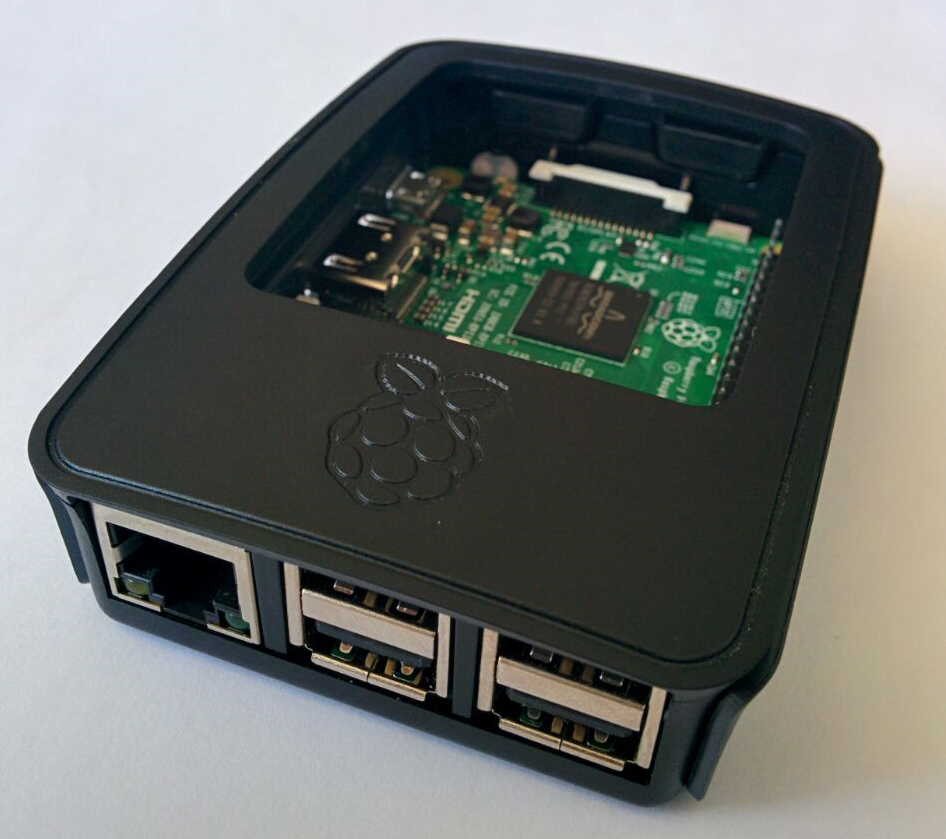
\includegraphics[width=0.65\textwidth]{./setup/raspi}
\caption{Raspberry Pi 3}
\label{Inf:Infraestructura}
\end{center}
\end{figure}


\section{Virtualización de la Raspberry}

Al inicio del proyecto no se disponía de una Raspberry para poder realizar las pruebas y se decidió emular la mediante qemu. 
Qemu es una aplicación que nos permite emular mediante máquinas virtuales gran parte de los sistemas operativos. 
Lo cual es realmente sencillo emular una imagen de Raspbian si no fuera por un detalle, como se comenta en el apartado ¿Qué es Docker? Docker necesita un sistema x64 o Linux kernel 3.8+ y Raspberry ejecuta un sistema ARM lo que conlleva que Docker no sea compatible a primera instancia con la Raspberry. 
La solución para este gran problema es la utilización de Hypriot, una imagen de Raspbian modificada con Docker instalado. 
La instalación de esta imagen  requiere hacer unos retoques ya que no es del todo compatible el kernel de qemu con el de la imagen de Hypriot. Cosa que aun que permite emular perfectamente la imagen con Docker, no nos permite el uso correcto. Por lo tanto se decidió apartar por completo la posibilidad de poder emular una Raspberry con Docker instalado ya que las incompatibilidades del kernel no lo permitían.

En el apéndice se podrá ver los pasos a seguir para la instalación y emulación de la imagen. 

\section{Raspberry y Docker}

Después de descartar completamente la opción de emular la imagen de la Raspberry se decidió probar en la Raspberry que disponía la empresa la imagen corria perfectamente. Y si, la imagen iba perfectamente y ejecutaba Docker sin ningún problema. Ahora el problema era la Raspberry, era el primer modelo el cual era viejo y no disponía de módulos para conexiones inalámbricas integrados por lo que se decidió aprovechando el lanzamiento de la nueva Raspberry 3 comprarla ya que si dispone de de conexiones inalámbrica. 

\subsection{Instalación de la imagen en la Raspberry}

La como se ha dicho, la imagen a la imagen de Raspbian no es posible instalar Docker de manera como lo haríamos en un sistema operativo como linux, es necesario una imagen la cual ya lo tenga instalado en nuestro caso utilizamos la imagen de Hypriot. La instalación se llevó a cabo de esta manera:

\begin{verbatim}
$ curl -sSL http://downloads.hypriot.com/docker-hypriot_1.8.2-1_armhf.deb 
>/tmp/docker-hypriot_1.8.2-1_armhf.deb
$ sudo dpkg -i /tmp/docker-hypriot_1.8.2-1_armhf.deb
$ rm -f /tmp/docker-hypriot_1.8.2-1_armhf.deb
$ sudo sh -c 'usermod -aG docker $SUDO_USER'
$ sudo systemctl enable docker.service
\end{verbatim}

\begin{itemize}
\item Primero descarga la imagen deseada y la montara en un directorio temporal.
\item Instalará los paquetes con el comando dpkg.
\item Borra el archivo comprimido.
\item Ejecutará el comando donde añade el usuario a un grupo docker. 
\item Pondrá en marcha el Daemon de Docker.  
\end{itemize}

Una vez tenemos la imagen preparada podremos hacer una copia binaria en una SD y ya estará lista para poder ser arrancada desde una Raspberry. 

\subsection{Creación de las imágenes de Docker}

Una vez tenemos la Raspberry lista, se pasará a la creación de las imágenes Docker para poder desplegar Aaaida.
En primer lugar se necesita un contenedor que contenga una base de datos en este caso, MongoDB. Para la creación de la imagen utilizaremos ya una creada y que esté en los repositorios de Docker Hub. Se necesita una imagen que sea compatible con ARM cosa que no resulta sencillo ya que la gran mayoría de las imágenes no están pensado para esta arquitectura y los pocos disponibles no estaban operativos. Otra restricción que teníamos era que debía ser una base de datos sin la necesidad de ingresar un usuario y su contraseña, cosa que no es habitual pero resultó una obligación en algunas imágenes.
Por lo tanto se utilizó la siguiente imagen de Docker Hub:

\begin{center}
\texttt{partlab/ubuntu-arm-mongodb}
\end{center}

La otra imagen que se utilizar será la propia de Aaaida, pero igual que la imagen de mongo debería ser compatible con una arquitectura ARM y al ser una aplicación propia de la empresa no se encontraría en repositorios público, tendríamos que crearla nosotros mediante un Dockerfile. 
En la siguiente figura se puede ver el Dockerfile que se utilizara para poder crear el contenedor con Aaaida.

\begin{verbatim}
FROM ioft/armhf-debian
RUN apt-get update; apt-get -y install curl
RUN set -ex \  
	&& for key in \    
		9554F04D7259F04124DE6B476D5A82AC7E37093B \ 
        94AE36675C464D64BAFA68DD7434390BDBE9B9C5 \
        0034A06D9D9B0064CE8ADF6BF1747F4AD2306D93 \ 
        FD3A5288F042B6850C66B31F09FE44734EB7990E \    
        71DCFD284A79C3B38668286BC97EC7A07EDE3FC1 \    
        DD8F2338BAE7501E3DD5AC78C273792F7D83545D \    
        B9AE9905FFD7803F25714661B63B535A4C206CA9 \    
        C4F0DFFF4E8C1A8236409D08E73BC641CC11F4C8 \  
	; 	do \  
		gpg --keyserver ha.pool.sks-keyservers.net --recv-keys "$key"; \  
	done

ENV NODE_VERSION 4.4.5

RUN curl -SLO 
"https://nodejs.org/dist/v$NODE_VERSION/node-v$NODE_VERSION-
linux-armv7l.tar.gz" \  
&& curl -SLO "https://nodejs.org/dist/v$NODE_VERSION/SHASUMS256.txt.asc" \  
&& gpg --batch --decrypt --output SHASUMS256.txt SHASUMS256.txt.asc \  
&& grep "node-v$NODE_VERSION-linux-armv7l.tar.gz\$" SHASUMS256.txt | 
sha256sum -c - \  
&& tar -xzf "node-v$NODE_VERSION-linux-armv7l.tar.gz" -C /usr/local 
--strip-components=1 \  
&& rm "node-v$NODE_VERSION-linux-armv7l.tar.gz" SHASUMS256.txt.asc 
SHASUMS256.txt

COPY scripts/rpi_docker/entrypoint /entrypoint
RUN mkdir /aaaida
WORKDIR /aaaida
CMD ["/entrypoint"]
EXPOSE 40000
COPY . /aaaida
\end{verbatim}

Al principio del Dockerfile se ve la acción \texttt{FROM} que ya fue explicada en la cual carga una imagen de una debian para ARM, como observación se puede detectar que la imagen del mongo es para Ubuntu ARM y la imagen base para la aplicación de Aaaida es una debian ARM, distribuciones de linux diferentes en los dos contenedores. Esto demuestra que cada contenedor es un ente aislado que no tiene que depender del resto de contenedores.
 
A continuación de declarar la imagen base, vienen una serie de acciones con la instrucción \texttt{RUN}, que nos permite ejecutar cualquier comando. En el primer caso que hace un update e instala el curl.
 
Las siguientes tres instrucciones de las cuales dos de ellas son un \texttt{RUN} y la restante un \texttt{ENV}, que configura las variables de entorno, son para poder instalar el Node.js en el contenedor para poder compilar el código de Aaaida.
 
Una vez instalado se utiliza la acción \texttt{COPY}, que como su nombre indica, copiara el contenido de un directorio en un directorio del contenedor.

Si seguimos se ve que crea un directorio con el nombre de \texttt{aaaida} y hace que ese directorio sea el directorio de trabajo con la instrucción \texttt{WORKDIR}.
 
Después Ejecutará \texttt{["/entrypoint"]} que al escribirlo en formato JSON la instrucción \texttt{CMD} ejecuta el contenido sin shell. El contenido de este script especifica los puertos, el host... de la aplicación. Se podrá ver su contenido en el apéndice.
 
Para terminar con las 2 últimas instrucciones, que son \texttt{EXPOSE} y \texttt{COPY}, la cual la primera indica los puertos que el contenedor tendrá activos y por los cuales escuchara. El segundo hará una copia desde el punto raíz donde se ejecute el Dockerfile en el directorio creado anteriormente de \texttt{aaaida}. 